%% SECTION HEADER /////////////////////////////////////////////////////////////////////////////////////
\section{Experimental Setup for the \ac{hsc} model validation}
\label{sec:setup}
%% SECTION CONTENT ////////////////////////////////////////////////////////////////////////////////////
\begin{figure}[H]
	\begin{center}
		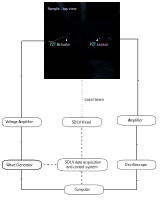
\includegraphics{Chapter_6/setup}
	\end{center}
	\caption{Experimental setup for the (1) \ac{sldv} measurement - dashed line and (2) PZT wave acquisition - solid line.}
	\label{fig:setup}
\end{figure}
The presented model of the \ac{hsc} was validated with results from two experimental studies.
The first one was performed for determination of the full wavefield of the propagating waves by the \ac{sldv} (Polytec PSV–400).
The second study was performed for wave acquisition by the \ac{pzt} sensor.
A schematic of the experimental scenarios is shown in Fig.~\ref{fig:setup}.

\ac{sldv} is a modern method for non-contact measurement of the vibration velocity of structure surface particles.
The principle of vibrometer operation is based on the Doppler effect, recording the change of frequency of the light beam reflected from the vibrating surface.
In laser vibrometry, the measurement of frequency change is realized by interferometer and analysis of both reference and measurement light beam.
The measuring system is additionally equipped with mirrors allowing to change the angle of the measuring beam, so it is possible to measure a grid of points on a surface automatically.
The \ac{sldv} setup is presented in Fig.~\ref{fig:sldv}.
\begin{figure}
	\begin{center}
		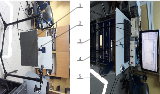
\includegraphics{Chapter_6/sldv}
	\end{center}
	\caption{The \ac{sldv} setup: 1 - laser sensor head, 2 - \ac{hsc} specimen, 3 - arbitrary wave generator, 4 - amplifier, 5 - data management system}
	\label{fig:sldv}
\end{figure}

The \ac{pzt} elastic wave generation and acquisition system is used to measure the voltage changes of transducers due to their mechanical deformation.
It is a point measurement at the point of sensor placement.
The following instruments are required to make the measurements: wave generator to prepare signal, amplifier to strengthen the excitation and recording signals, oscilloscope and central management unit.
The setup used for measurements is shown in Fig.~\ref{fig:pzt_setup}.
\begin{figure}[t]
	\begin{center}
		\includegraphics{Chapter_6/pzt_setup}
	\end{center}
	\caption{The \ac{pzt} setup,(\textbf{a}) elastic wave generation and acquisition instruments:  1 - arbitrary wave generator, 2 - amplifier, 3 - oscilloscope, 4 - data management unit, (\textbf{b}) the specimen held in the environmental chamber.}
	\label{fig:pzt_setup}
\end{figure}

Both methods have some advantages and disadvantages, which are given in the Table~\ref{tab:method_comp}.
\begin{table}[H]
	\small
	\tabcolsep=0.75cm
	%\centering
	\caption{\label{tab:method_comp}Comparison of the methods for elastic wave propagation measurement.}
	\begin{tabular}{p{0.1\textwidth}>{\raggedright}p{0.3\textwidth}>{\raggedright \arraybackslash}p{0.3\textwidth}}
		\toprule
		\textbf{Method} &\textbf{Advantages} & \textbf{Disadvantages}\\\midrule
		\multirow{5}{*}{\ac{sldv}}   & \tabitem automatic fullfield scanning & \tabitem high-cost equipment\\ & \tabitem non-contact measurement & \tabitem additional setup for signal generation \\
		& \tabitem \ac{3d} velocity vector & \tabitem special foil stuck to the measuring surface needed to avoid scattering of the laser beam\\
		& & \tabitem high noise-to-signal ratio\\
		& & \tabitem relatively large space need for measurements \\
		& & \tabitem special sample mounting for repeatability of measurements \\
		\midrule
		\multirow{5}{*}{\ac{pzt}} & \tabitem low-lost instruments & \tabitem spot measurement\\
		& \tabitem high repeatability of measurements & \tabitem displacements vector correlated with the sensor polarization\\
		& \tabitem measurements on the sample in motion & \tabitem cumbersome wiring\\
		& \tabitem generation and recording signals with the same setup & \tabitem sensitive to electric and magnetic fields\\		
		\bottomrule
	\end{tabular}
\end{table}


The sample was fabricated under workshop conditions from the components described in Section~\ref{sec:sample}.
Before applying the two-ingredient glue (Loctite EA3479B), the bottom surface of the skin was cleaned and degreased with the solver (Loctite SF7063).
The adhesive curing took 48 hours under a distributed load at ambient temperature.
The subject of the parametric study was the effect of the disbond size on the propagating \ac{gw}.
After a reference measurement was made on an intact sample, several measurements were taken for the subsequent damage introduced on the same specimen.
The rectangular area of the core was detached from the adhesive at the center of the plate using a sharp hooked tool.
The damage width varied in range \(w_D=\left [10, 30, 50, 70, 100, 120 \right ]\) mm, while its fixed length was \(l_d = 175\) mm.

The \(N_c=5\) cycle Hann windowed signal at carrier frequencies \(f_c=[50,100,150]\) kHz was generated using an arbitrary waveform generator (National Instruments, PXI 5413).
The signal was amplified 3.5 times and supplied to the \ac{pzt} actuator (Noliac, NCE51).
Each measurement was conducted under \(20^{\circ}\)C controlled in the environmental chamber (DM 600C, Angelantoni Test Technologies Srl) and averaged 20~times in order to improve the signal to noise ratio.